\documentclass[8pt,a4paper,compress]{beamer}

\usepackage{/home/siyer/lib/slides}
\usepackage{tabularx}

\newcolumntype{L}[1]{>{\raggedright\arraybackslash}p{#1}}
\newcolumntype{C}[1]{>{\centering\arraybackslash}p{#1}}
\newcolumntype{R}[1]{>{\raggedleft\arraybackslash}p{#1}}

\title{Compilation}
\date{}

\begin{document}
\begin{frame}
\vfill
\titlepage
\end{frame}

\section{Compilers}
\begin{frame}[fragile]
\pause

A compiler translates a high-level source language program into a low-level target language program

\begin{center}
\visible<2->{
\begin{tikzpicture}
\footnotesize
\begin{scope}[->,thin,
	   node distance=0.5cm,
  	   block1/.style={rectangle,draw,align=center},
	   block2/.style={rectangle,align=center}]
\node [block2] (1) {Source \\ Language \\ Program};
\node [block1] (2) [right=of 1] {Compiler};
\node [block2] (3) [right=of 2] {Target \\ Language \\ Program};
\path (1) edge node [above] {} (2);
\path (2) edge node [above] {} (3);
\end{scope}
\end{tikzpicture}
}
\end{center}

\pause\bigskip

Examples of source language: C, Java

\pause\bigskip

Examples of target language: MIPS instructions, JVM instructions
\end{frame}

\begin{frame}[fragile]
\pause

The description of a programming language consists of
\begin{itemize}
\pause
\item Tokens (aka lexemes)

\pause
\item Syntax of constructs such as classes, methods, statements, and expressions

\pause
\item Meaning (aka semantics) of the constructs
\end{itemize}
\end{frame}

\begin{frame}[fragile]
\pause

A machine's instruction set and its behavior is referred to as its architecture

\pause\bigskip

Examples of architectures
\begin{itemize}
\pause
\item Intel i386: a complex instruction set computer (CISC)

\pause
\item MIPS: a reduced instruction set computer (RISC)

\pause
\item Java Virtual Machine (JVM): a virtual machine
\end{itemize}
\end{frame}

\begin{frame}[fragile]
\pause

An interpreter executes a high-level source language program directly

\begin{center}
\visible<2->{
\begin{tikzpicture}
\footnotesize
\begin{scope}[->,thin,
	   node distance=0.5cm,
	   block1/.style={rectangle,draw,align=center},
	   block2/.style={rectangle,align=center}]
\node [block2] (1) {Source \\ Language \\ Program};
\node [block1] (2) [right=of 1] {Interpreter};
\node [block2] (3) [right=of 2] {Results};
\path (1) edge node [above] {} (2);
\path (2) edge node [above] {} (3);
\end{scope}
\end{tikzpicture}
}
\end{center}

\pause\bigskip

Examples of interpreters: Bash, Python
\end{frame}

\section{Why Study Compilers?}
\begin{frame}[fragile]
\pause

Compilers are larger programs than the ones you have written so far

\pause\bigskip

Compilers make use of all those things you have learned about earlier

\pause\bigskip

You learn a lot about the source language (in our case, Java)

\pause\bigskip

You learn a lot about the target machine (in our case, JVM and MIPS)

\pause\bigskip

Compilers are still being written for new languages and targeted to new architectures

\pause\bigskip

There is a good mix of theory and practice

\pause\bigskip

Compiler writing is a case study in software engineering

\pause\bigskip

Compilers are programs and writing programs is fun
\end{frame}

\section{The Phases of Compilation}
\begin{frame}[fragile]
\pause

A compiler can be broken into a front end and a back end

\begin{center}
\visible<2->{
\begin{tikzpicture}
\footnotesize
\begin{scope}[->,thin,
	   node distance=0.5cm,
  	   block1/.style={rectangle,draw,align=center},
	   block2/.style={rectangle,align=center}]
\node [block2] (1) {Source \\ Language \\ Program};
\node [block1] (2) [right=of 1] {Front End};
\node [block2] (3) [right=of 2] {IR};
\node [block1] (4) [right=of 3] {Back End};
\node [block2] (5) [right=of 4] {Target \\ Language \\ Program};
\path (1) edge node [above] {} (2);
\path (2) edge node [above] {} (3);
\path (3) edge node [above] {} (4);
\path (4) edge node [above] {} (5);
\end{scope}
\end{tikzpicture}
}
\end{center}

\pause\bigskip

The front end analyzes the source language program for its meaning and produces an intermediate representation (IR) of the program

\pause\bigskip

The front end is source language dependent and target language independent

\pause\bigskip

The back end takes the IR and synthesizes a target language program

\pause\bigskip

The back end is target language dependent and source language independent
\end{frame}

\begin{frame}[fragile]
\pause

The front end can be decomposed into a sequence of analysis phases

\begin{center}
\visible<2->{
\begin{tikzpicture}
\footnotesize
\begin{scope}[->,thin,
	   node distance=0.5cm,
  	   block1/.style={rectangle,draw,align=center},
	   block2/.style={rectangle,align=center}]
\node [block2] (1) {Source \\ Language \\ Program};
\node [block1] (2) [right=of 1] {Scanner};
\node [block2] (3) [right=of 2] {Tokens};
\node [block1] (4) [right=of 3] {Parser};
\node [block2] (5) [right=of 4] {AST};
\node [block1] (6) [right=of 5] {Semantics};
\node [block2] (7) [right=of 6] {IR};
\path (1) edge node [above] {} (2);
\path (2) edge node [above] {} (3);
\path (3) edge node [above] {} (4);
\path (4) edge node [above] {} (5);
\path (5) edge node [above] {} (6);
\path (6) edge node [above] {} (7);
\end{scope}
\end{tikzpicture}
}
\end{center}

\pause\bigskip

The scanner breaks the input stream of characters into a sequence of tokens

\pause\bigskip

The parser takes the sequence of tokens and parses it against a grammar to produce an abstract syntax tree (AST)

\pause\bigskip

The semantics phase
\begin{itemize}
\pause
\item Declares names in a symbol table

\pause
\item Looks up names as they are referenced to determine their types 

\pause
\item Assigns types to expressions and checks the validity of types

\pause
\item Does certain amount of storage analysis 
\end{itemize}
\end{frame}

\begin{frame}[fragile]
\pause

The back end can be decomposed into a sequence of synthesis phases

\begin{center}
\visible<2->{
\begin{tikzpicture}
\footnotesize
\begin{scope}[->,thin,
	   node distance=0.5cm,
  	   block1/.style={rectangle,draw,align=center},
	   block2/.style={rectangle,align=center}]
\node [block2] (1) {IR};
\node [block1] (2) [right=of 1] {Codegen};
\node [block2] (3) [right=of 2] {Target \\ Language \\ Instructions};
\node [block1] (4) [right=of 3] {Peephole};
\node [block2] (5) [right=of 4] {Better \\ Target \\ Language \\ Instructions};
\node [block1] (6) [right=of 5] {Object};
\node [block2] (7) [right=of 6] {Target \\ Language \\ Program};
\path (1) edge node [above] {} (2);
\path (2) edge node [above] {} (3);
\path (3) edge node [above] {} (4);
\path (4) edge node [above] {} (5);
\path (5) edge node [above] {} (6);
\path (6) edge node [above] {} (7);
\end{scope}
\end{tikzpicture}
}
\end{center}

\pause\bigskip

The code generation phase chooses what target machine instructions to generate

\pause\bigskip

The peephole phase scans through the generated instructions locally for wasteful instructions such as branches to branches and unnecessary load/store pairs

\pause\bigskip

The object phase links together modules produced in code generation and constructs a single target language program
\end{frame}

\begin{frame}[fragile]
\pause

A compiler sometimes has an optimizer between the front end and the back end

\begin{center}
\visible<2->{
\begin{tikzpicture}
\footnotesize
\begin{scope}[->,thin,
	   node distance=0.5cm,
  	   block1/.style={rectangle,draw,align=center},
	   block2/.style={rectangle,align=center}]
\node [block2] (1) {Source \\ Language \\ Program};
\node [block1] (2) [right=of 1] {Front End};
\node [block2] (3) [right=of 2] {IR};
\node [block1] (4) [right=of 3] {Optimizer};
\node [block2] (5) [right=of 4] {Better \\ IR};
\node [block1] (6) [right=of 5] {Back End};
\node [block2] (7) [right=of 6] {Target \\ Language \\ Program};
\path (1) edge node [above] {} (2);
\path (2) edge node [above] {} (3);
\path (3) edge node [above] {} (4);
\path (4) edge node [above] {} (5);
\path (5) edge node [above] {} (6);
\path (6) edge node [above] {} (7);
\end{scope}
\end{tikzpicture}
}
\end{center}

\pause\bigskip

The optimizer might
\begin{itemize}
\pause
\item Eliminate common sub-expressions

\pause
\item Perform constant folding

\pause
\item Lift loop invariants out of loops

\pause
\item Perform strength reduction
\end{itemize}
\end{frame}

\begin{frame}[fragile]
\pause

Advantages of separating the front end from the back end
\begin{itemize}
\pause
\item It is easier to understand (and implement) smaller programs

\pause
\item Several individuals or teams can work concurrently on separate parts

\pause
\item Enables a certain amount of code re-use

\bigskip
\begin{minipage}[t]{\linewidth}
\begin{center}
\begin{overprint}
\onslide<6|handout:1>
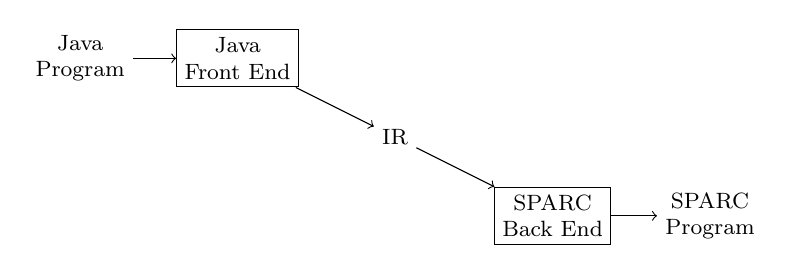
\begin{tikzpicture}
\footnotesize
\begin{scope}[->,thin,
              block1/.style={rectangle,draw,align=center},
	          block2/.style={rectangle,align=center}]
    \node [block2] (1) at (0,2) {Java \\ Program};
%    \node [block2] (2) at (0,0) {C \\ Program};
    \node [block1] (3) at (2,2) {Java \\ Front End};
%    \node [block1] (4) at (2,0) {C \\ Front End};
%    \node [block1] (5) at (6,2) {Intel \\ Back End};
    \node [block1] (6) at (6,0) {SPARC \\ Back End};
%    \node [block2] (7) at (8,2) {Intel Core Duo \\ Program};
    \node [block2] (8) at (8,0) {SPARC \\ Program};
    \node [block2] (9) at (4,1) {IR};
    \path (1) edge node [above] {} (3);
%    \path (2) edge node [above] {} (4);
%    \path (5) edge node [above] {} (7);
    \path (6) edge node [above] {} (8);
    \path (3) edge node [above] {} (9);
%    \path (4) edge node [above] {} (9);
%    \path (9) edge node [above] {} (5);
    \path (9) edge node [above] {} (6);
\end{scope}
\end{tikzpicture}

\onslide<7|handout:2>
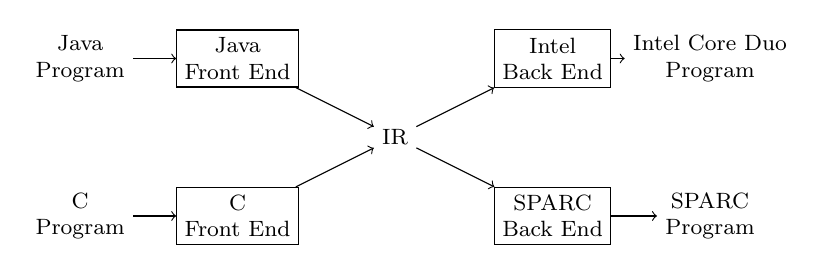
\begin{tikzpicture}
\footnotesize
\begin{scope}[->,thin,
              block1/.style={rectangle,draw,align=center},
	          block2/.style={rectangle,align=center}]
    \node [block2] (1) at (0,2) {Java \\ Program};
    \node [block2] (2) at (0,0) {C \\ Program};
    \node [block1] (3) at (2,2) {Java \\ Front End};
    \node [block1] (4) at (2,0) {C \\ Front End};
    \node [block1] (5) at (6,2) {Intel \\ Back End};
    \node [block1] (6) at (6,0) {SPARC \\ Back End};
    \node [block2] (7) at (8,2) {Intel Core Duo \\ Program};
    \node [block2] (8) at (8,0) {SPARC \\ Program};
    \node [block2] (9) at (4,1) {IR};
    \path (1) edge node [above] {} (3);
    \path (2) edge node [above] {} (4);
    \path (5) edge node [above] {} (7);
    \path (6) edge node [above] {} (8);
    \path (3) edge node [above] {} (9);
    \path (4) edge node [above] {} (9);
    \path (9) edge node [above] {} (5);
    \path (9) edge node [above] {} (6);
\end{scope}
\end{tikzpicture} 
\end{overprint}
\end{center}
\end{minipage}
\end{itemize}
\end{frame}

\begin{frame}[fragile]
\pause

We will implement a compiler called \jmm to compile a non-trivial subset of Java, also called \jmm

\pause\bigskip

In the first instance, we will target the JVM, a stack-based architecture

\pause\bigskip

Compiling a \jmm program \lstinline{P.java} for JVM
\begin{tcolorbox}[enhanced,drop shadow southwest,sharp corners,size=fbox,colback=black]
\begin{lstlisting}[style=terminal]
$ j-- P.java
\end{lstlisting}
\end{tcolorbox}

\pause\bigskip

Running the JVM program \lstinline{P.class}
\begin{tcolorbox}[enhanced,drop shadow southwest,sharp corners,size=fbox,colback=black]
\begin{lstlisting}[style=terminal]
$ java P
\end{lstlisting}
\end{tcolorbox}

\pause\bigskip

Besides the JVM, we will also target the MIPS machine, a register-based architecture

\pause\bigskip

Compiling a \jmm program \lstinline{P.java} for MIPS
\begin{tcolorbox}[enhanced,drop shadow southwest,sharp corners,size=fbox,colback=black]
\begin{lstlisting}[style=terminal]
$ j-- -s naive P.java
\end{lstlisting}
\end{tcolorbox}

\pause\bigskip

Running the MIPS program \lstinline{P.s}

\begin{tcolorbox}[enhanced,drop shadow southwest,sharp corners,size=fbox,colback=black]
\begin{lstlisting}[style=terminal]
$ spim -f P.s
\end{lstlisting}
\end{tcolorbox}
\end{frame}

\section{Overview of the \protect \jmm to JVM Compiler}
\begin{frame}[fragile]
\pause

\jmm is an object-oriented programming language, supporting classes, methods, fields, message expressions, and a variety of statements, expressions and primitive types

\pause\bigskip

The \jmm compiler is organized in an object-oriented fashion

\bigskip

\begin{center}
\begin{overprint}
\onslide<4|handout:1>
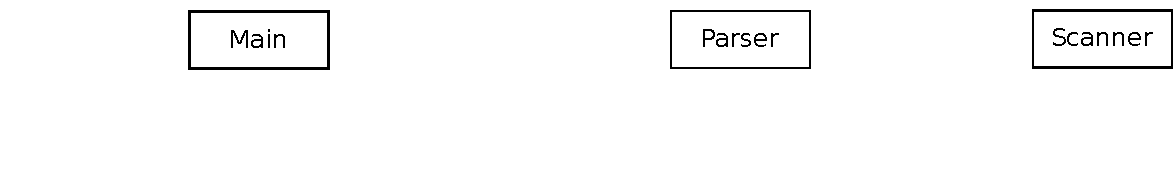
\includegraphics[scale=0.45]{figures/organization1.pdf}

\onslide<5|handout:2>
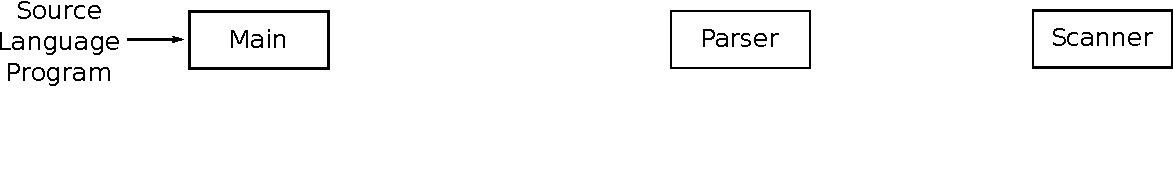
\includegraphics[scale=0.45]{figures/organization2.pdf}

\onslide<6|handout:3>
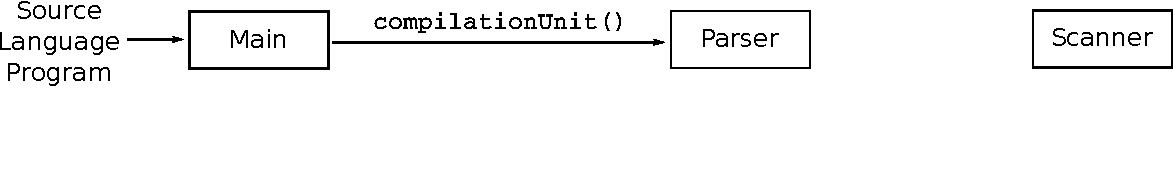
\includegraphics[scale=0.45]{figures/organization3.pdf}

\onslide<7|handout:4>
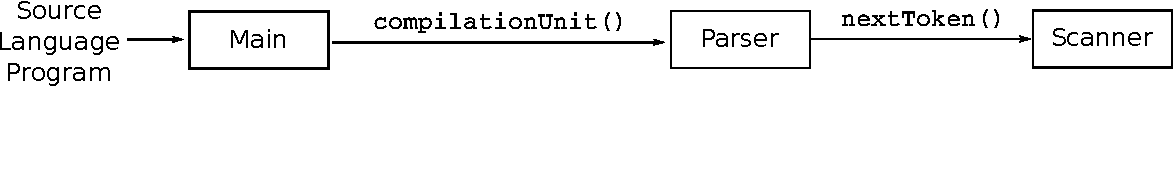
\includegraphics[scale=0.45]{figures/organization4.pdf}

\onslide<8|handout:5>
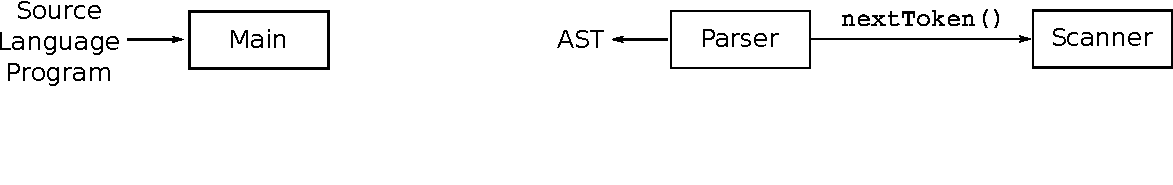
\includegraphics[scale=0.45]{figures/organization5.pdf}

\onslide<9|handout:6>
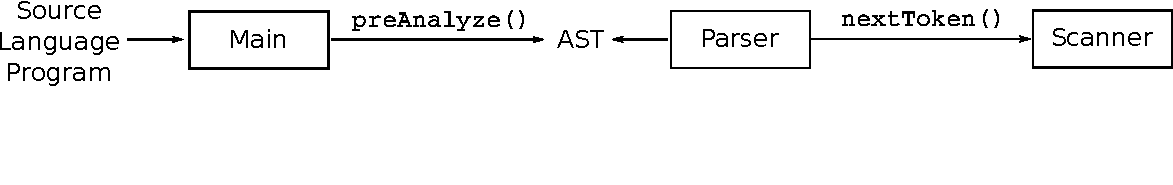
\includegraphics[scale=0.45]{figures/organization6.pdf}

\onslide<10|handout:7>
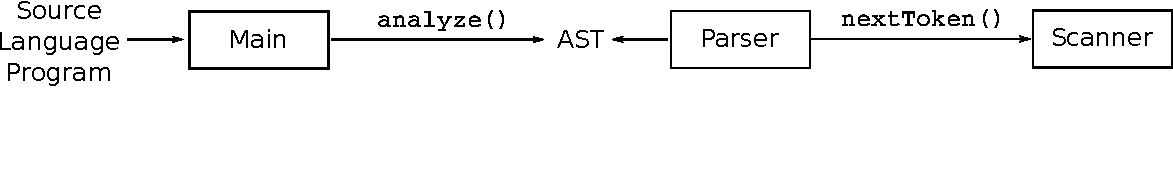
\includegraphics[scale=0.45]{figures/organization7.pdf}

\onslide<11|handout:8>
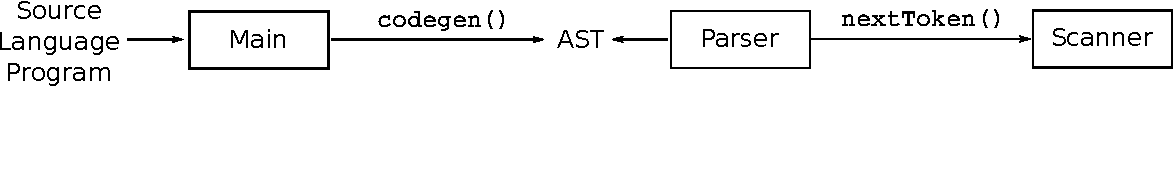
\includegraphics[scale=0.45]{figures/organization8.pdf}

\onslide<12|handout:9>
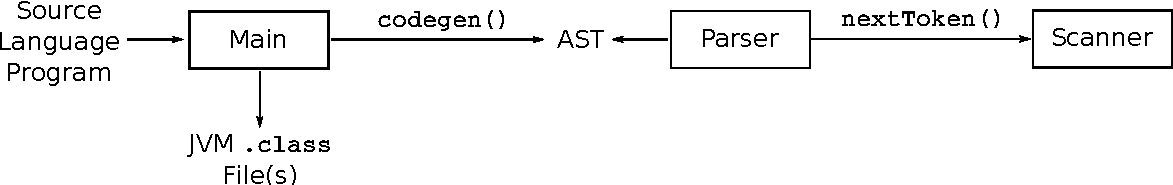
\includegraphics[scale=0.45]{figures/organization9.pdf}
\end{overprint}
\end{center}
\end{frame}

\begin{frame}[fragile]
\pause

The scanner breaks down a \jmm program into a sequence of tokens

\pause\bigskip

Consider the program

\pause\smallskip

\begin{tcolorbox}[enhanced,drop shadow southwest,sharp corners,size=fbox,colback=white,fontlower=\small\ttfamily,collower=silver100]

\begin{lstlisting}[language=Java,style=focusin]
package pass;

import java.lang.System;

public class HelloWorld {
    // The only method.
    public static void main(String[] args) {
        System.out.println("Hello, World!");
    }
}
\end{lstlisting}
\end{tcolorbox}

\pause\smallskip

The program is broken down into tokens \lstinline{package}, \lstinline{pass}, \lstinline{;}, \lstinline{import}, \lstinline{java}, \lstinline{.}, and so on

\pause\bigskip

Tokens such as \lstinline{java} and \lstinline{HelloWorld} are \lstinline{IDENTIFIER} tokens, carrying along their images (\lstinline{"java"} and \lstinline{"HelloWorld"}) as attributes

\pause\bigskip

Tokens such as \lstinline{package} and \lstinline{import} are reserved words having the unique names such as \lstinline{PACKAGE} and \lstinline{IMPORT}

\pause\bigskip

Operators and separators such as \lstinline{+} and \lstinline{;} have distinct names such as \lstinline{PLUS} and \lstinline{SEMI}

\pause\bigskip

Literals such as \lstinline{"Hello, World!"} comprise a single token such as \lstinline{STRING_LITERAL}

\pause\bigskip

Comments are scanned and completely ignored
\end{frame}

\begin{frame}[fragile]


\onslide<2->
The parser validates the syntax of a \jmm program against the \jmm grammar and represents the program as an AST

\bigskip

\onslide<3->
In the first instance, the parser is hand-crafted from the grammar, to parse programs by a technique known as recursive descent

\bigskip

\onslide<4->
Consider the grammar rule describing a compilation unit

\smallskip

\begin{overprint}
\onslide<5|handout:1>
\begin{tcolorbox}[enhanced,drop shadow southwest,sharp corners,size=fbox,colback=white,fontlower=\small\ttfamily,collower=silver900]

\begin{lstlisting}[language={},style=focusin]
compilationUnit ::= [PACKAGE qualifiedIdentifier SEMI]
                    {IMPORT  qualifiedIdentifier SEMI}
                    {typeDeclaration} 
                    EOF
\end{lstlisting}

\tcblower
\begin{minipage}[t][.25cm][t]{\textwidth}

\end{minipage}
\end{tcolorbox}

\onslide<6|handout:2>
\begin{tcolorbox}[enhanced,drop shadow southwest,sharp corners,size=fbox,colback=white,fontlower=\small\ttfamily,collower=silver900]

\begin{lstlisting}[language={},style=focusin,backgroundcolor=\color{lime100}]
compilationUnit ::= [PACKAGE qualifiedIdentifier SEMI]
\end{lstlisting}
\begin{lstlisting}[language={},style=focusout]
                    {IMPORT  qualifiedIdentifier SEMI}
                    {typeDeclaration} 
                    EOF
\end{lstlisting}

\tcblower
\begin{minipage}[t][.25cm][t]{\textwidth}
optional package statement
\end{minipage}
\end{tcolorbox}

\onslide<7|handout:3>
\begin{tcolorbox}[enhanced,drop shadow southwest,sharp corners,size=fbox,colback=white,fontlower=\small\ttfamily,collower=silver900]

\begin{lstlisting}[language={},style=focusout]
compilationUnit ::= [PACKAGE qualifiedIdentifier SEMI]
\end{lstlisting}
\begin{lstlisting}[language={},style=focusin,backgroundcolor=\color{lime100}]
                    {IMPORT  qualifiedIdentifier SEMI}
\end{lstlisting}
\begin{lstlisting}[language={},style=focusout]
                    {typeDeclaration} 
                    EOF
\end{lstlisting}

\tcblower
\begin{minipage}[t][.25cm][t]{\textwidth}
zero or more import statements
\end{minipage}
\end{tcolorbox}

\onslide<8|handout:4>
\begin{tcolorbox}[enhanced,drop shadow southwest,sharp corners,size=fbox,colback=white,fontlower=\small\ttfamily,collower=silver900]

\begin{lstlisting}[language={},style=focusout]
compilationUnit ::= [PACKAGE qualifiedIdentifier SEMI]
                    {IMPORT  qualifiedIdentifier SEMI}
\end{lstlisting}
\begin{lstlisting}[language={},style=focusin,backgroundcolor=\color{lime100}]
                    {typeDeclaration} 
\end{lstlisting}
\begin{lstlisting}[language={},style=focusout]
                    EOF
\end{lstlisting}
\tcblower
\begin{minipage}[t][.25cm][t]{\textwidth}
zero or more type (class) declarations
\end{minipage}
\end{tcolorbox}

\onslide<9|handout:5>
\begin{tcolorbox}[enhanced,drop shadow southwest,sharp corners,size=fbox,colback=white,fontlower=\small\ttfamily,collower=silver900]

\begin{lstlisting}[language={},style=focusout]
compilationUnit ::= [PACKAGE qualifiedIdentifier SEMI]
                    {IMPORT  qualifiedIdentifier SEMI}
                    {typeDeclaration} 
\end{lstlisting}
\begin{lstlisting}[language={},style=focusin,backgroundcolor=\color{lime100}]
                    EOF
\end{lstlisting}

\tcblower
\begin{minipage}[t][.25cm][t]{\textwidth}
end of file
\end{minipage}
\end{tcolorbox}
\end{overprint}
\end{frame}

\begin{frame}[fragile]
\pause

A compilation unit is parsed by the method \lstinline{compilationUnit()} defined in \lstinline{Parser.java}

\smallskip

\begin{overprint}
\onslide<2|handout:1>
\begin{tcolorbox}[enhanced,drop shadow southwest,sharp corners,size=fbox,colback=white,fontlower=\small\ttfamily,collower=silver900]

\begin{lstlisting}[language=Java,style=focusin]
    public JCompilationUnit compilationUnit() {
        int line = scanner.token().line();
        TypeName packageName = null;
        if (have(PACKAGE)) {
            packageName = qualifiedIdentifier();
            mustBe(SEMI);
        }
        ArrayList<TypeName> imports = new ArrayList<TypeName>();
        while (have(IMPORT)) {
            imports.add(qualifiedIdentifier());
            mustBe(SEMI);
        }
        ArrayList<JAST> typeDeclarations = new ArrayList<JAST>();
        while (!see(EOF)) {
            JAST typeDeclaration = typeDeclaration();
            if (typeDeclaration != null) {
                typeDeclarations.add(typeDeclaration);
            }
        }
        mustBe(EOF);
        return new JCompilationUnit(scanner.fileName(), line, 
            packageName, imports, typeDeclarations);
    }
\end{lstlisting}

\tcblower
\begin{minipage}[t][.25cm][t]{\textwidth}

\end{minipage}
\end{tcolorbox}

\onslide<3|handout:2>
\begin{tcolorbox}[enhanced,drop shadow southwest,sharp corners,size=fbox,colback=white,fontlower=\small\ttfamily,collower=silver900]

\begin{lstlisting}[language=Java,style=focusin,backgroundcolor=\color{lime100}]
    public JCompilationUnit compilationUnit() {
\end{lstlisting}
\begin{lstlisting}[language=Java,style=focusout]
        int line = scanner.token().line();
        TypeName packageName = null;
        if (have(PACKAGE)) {
            packageName = qualifiedIdentifier();
            mustBe(SEMI);
        }
        ArrayList<TypeName> imports = new ArrayList<TypeName>();
        while (have(IMPORT)) {
            imports.add(qualifiedIdentifier());
            mustBe(SEMI);
        }
        ArrayList<JAST> typeDeclarations = new ArrayList<JAST>();
        while (!see(EOF)) {
            JAST typeDeclaration = typeDeclaration();
            if (typeDeclaration != null) {
                typeDeclarations.add(typeDeclaration);
            }
        }
        mustBe(EOF);
        return new JCompilationUnit(scanner.fileName(), line, 
            packageName, imports, typeDeclarations);
    }
\end{lstlisting}

\tcblower
\begin{minipage}[t][.25cm][t]{\textwidth}
parse a compilation unit and return an AST representation for it
\end{minipage}
\end{tcolorbox}

\onslide<4|handout:3>
\begin{tcolorbox}[enhanced,drop shadow southwest,sharp corners,size=fbox,colback=white,fontlower=\small\ttfamily,collower=silver900]

\begin{lstlisting}[language=Java,style=focusout]
    public JCompilationUnit compilationUnit() {
\end{lstlisting}
\begin{lstlisting}[language=Java,style=focusin,backgroundcolor=\color{lime100}]
        int line = scanner.token().line();
\end{lstlisting}
\begin{lstlisting}[language=Java,style=focusout]
        TypeName packageName = null;
        if (have(PACKAGE)) {
            packageName = qualifiedIdentifier();
            mustBe(SEMI);
        }
        ArrayList<TypeName> imports = new ArrayList<TypeName>();
        while (have(IMPORT)) {
            imports.add(qualifiedIdentifier());
            mustBe(SEMI);
        }
        ArrayList<JAST> typeDeclarations = new ArrayList<JAST>();
        while (!see(EOF)) {
            JAST typeDeclaration = typeDeclaration();
            if (typeDeclaration != null) {
                typeDeclarations.add(typeDeclaration);
            }
        }
        mustBe(EOF);
        return new JCompilationUnit(scanner.fileName(), line, 
            packageName, imports, typeDeclarations);
    }
\end{lstlisting}

\tcblower
\begin{minipage}[t][.25cm][t]{\textwidth}
get line number of current token
\end{minipage}
\end{tcolorbox}

\onslide<5|handout:4>
\begin{tcolorbox}[enhanced,drop shadow southwest,sharp corners,size=fbox,colback=white,fontlower=\small\ttfamily,collower=silver900]

\begin{lstlisting}[language=Java,style=focusout]
    public JCompilationUnit compilationUnit() {
        int line = scanner.token().line();
\end{lstlisting}
\begin{lstlisting}[language=Java,style=focusin,backgroundcolor=\color{lime100}]
        TypeName packageName = null;
        if (have(PACKAGE)) {
            packageName = qualifiedIdentifier();
            mustBe(SEMI);
        }
\end{lstlisting}
\begin{lstlisting}[language=Java,style=focusout]
        ArrayList<TypeName> imports = new ArrayList<TypeName>();
        while (have(IMPORT)) {
            imports.add(qualifiedIdentifier());
            mustBe(SEMI);
        }
        ArrayList<JAST> typeDeclarations = new ArrayList<JAST>();
        while (!see(EOF)) {
            JAST typeDeclaration = typeDeclaration();
            if (typeDeclaration != null) {
                typeDeclarations.add(typeDeclaration);
            }
        }
        mustBe(EOF);
        return new JCompilationUnit(scanner.fileName(), line, 
            packageName, imports, typeDeclarations);
    }
\end{lstlisting}

\tcblower
\begin{minipage}[t][.25cm][t]{\textwidth}
parse optional package statement
\end{minipage}
\end{tcolorbox}

\onslide<6|handout:5>
\begin{tcolorbox}[enhanced,drop shadow southwest,sharp corners,size=fbox,colback=white,fontlower=\small\ttfamily,collower=silver900]

\begin{lstlisting}[language=Java,style=focusout]
    public JCompilationUnit compilationUnit() {
        int line = scanner.token().line();
        TypeName packageName = null;
        if (have(PACKAGE)) {
            packageName = qualifiedIdentifier();
            mustBe(SEMI);
        }
\end{lstlisting}
\begin{lstlisting}[language=Java,style=focusin,backgroundcolor=\color{lime100}]
        ArrayList<TypeName> imports = new ArrayList<TypeName>();
        while (have(IMPORT)) {
            imports.add(qualifiedIdentifier());
            mustBe(SEMI);
        }
\end{lstlisting}
\begin{lstlisting}[language=Java,style=focusout]
        ArrayList<JAST> typeDeclarations = new ArrayList<JAST>();
        while (!see(EOF)) {
            JAST typeDeclaration = typeDeclaration();
            if (typeDeclaration != null) {
                typeDeclarations.add(typeDeclaration);
            }
        }
        mustBe(EOF);
        return new JCompilationUnit(scanner.fileName(), line, 
            packageName, imports, typeDeclarations);
    }
\end{lstlisting}

\tcblower
\begin{minipage}[t][.25cm][t]{\textwidth}
parse zero or more import statements
\end{minipage}
\end{tcolorbox}

\onslide<7|handout:6>
\begin{tcolorbox}[enhanced,drop shadow southwest,sharp corners,size=fbox,colback=white,fontlower=\small\ttfamily,collower=silver900]

\begin{lstlisting}[language=Java,style=focusout]
    public JCompilationUnit compilationUnit() {
        int line = scanner.token().line();
        TypeName packageName = null;
        if (have(PACKAGE)) {
            packageName = qualifiedIdentifier();
            mustBe(SEMI);
        }
        ArrayList<TypeName> imports = new ArrayList<TypeName>();
        while (have(IMPORT)) {
            imports.add(qualifiedIdentifier());
            mustBe(SEMI);
        }
\end{lstlisting}
\begin{lstlisting}[language=Java,style=focusin,backgroundcolor=\color{lime100}]
        ArrayList<JAST> typeDeclarations = new ArrayList<JAST>();
        while (!see(EOF)) {
            JAST typeDeclaration = typeDeclaration();
            if (typeDeclaration != null) {
                typeDeclarations.add(typeDeclaration);
            }
        }
\end{lstlisting}
\begin{lstlisting}[language=Java,style=focusout]
        mustBe(EOF);
        return new JCompilationUnit(scanner.fileName(), line, 
            packageName, imports, typeDeclarations);
    }
\end{lstlisting}

\tcblower
\begin{minipage}[t][.25cm][t]{\textwidth}
parse zero or more type (class) declarations
\end{minipage}
\end{tcolorbox}

\onslide<8|handout:7>
\begin{tcolorbox}[enhanced,drop shadow southwest,sharp corners,size=fbox,colback=white,fontlower=\small\ttfamily,collower=silver900]

\begin{lstlisting}[language=Java,style=focusout]
    public JCompilationUnit compilationUnit() {
        int line = scanner.token().line();
        TypeName packageName = null;
        if (have(PACKAGE)) {
            packageName = qualifiedIdentifier();
            mustBe(SEMI);
        }
        ArrayList<TypeName> imports = new ArrayList<TypeName>();
        while (have(IMPORT)) {
            imports.add(qualifiedIdentifier());
            mustBe(SEMI);
        }
        ArrayList<JAST> typeDeclarations = new ArrayList<JAST>();
        while (!see(EOF)) {
            JAST typeDeclaration = typeDeclaration();
            if (typeDeclaration != null) {
                typeDeclarations.add(typeDeclaration);
            }
        }
\end{lstlisting}
\begin{lstlisting}[language=Java,style=focusin,backgroundcolor=\color{lime100}]
        mustBe(EOF);
\end{lstlisting}
\begin{lstlisting}[language=Java,style=focusout]
        return new JCompilationUnit(scanner.fileName(), line, 
            packageName, imports, typeDeclarations);
    }
\end{lstlisting}

\tcblower
\begin{minipage}[t][.25cm][t]{\textwidth}
parse end of file
\end{minipage}
\end{tcolorbox}

\onslide<9|handout:8>
\begin{tcolorbox}[enhanced,drop shadow southwest,sharp corners,size=fbox,colback=white,fontlower=\small\ttfamily,collower=silver900]

\begin{lstlisting}[language=Java,style=focusout]
    public JCompilationUnit compilationUnit() {
        int line = scanner.token().line();
        TypeName packageName = null;
        if (have(PACKAGE)) {
            packageName = qualifiedIdentifier();
            mustBe(SEMI);
        }
        ArrayList<TypeName> imports = new ArrayList<TypeName>();
        while (have(IMPORT)) {
            imports.add(qualifiedIdentifier());
            mustBe(SEMI);
        }
        ArrayList<JAST> typeDeclarations = new ArrayList<JAST>();
        while (!see(EOF)) {
            JAST typeDeclaration = typeDeclaration();
            if (typeDeclaration != null) {
                typeDeclarations.add(typeDeclaration);
            }
        }
        mustBe(EOF);
\end{lstlisting}
\begin{lstlisting}[language=Java,style=focusin,backgroundcolor=\color{lime100}]
        return new JCompilationUnit(scanner.fileName(), line, 
            packageName, imports, typeDeclarations);
\end{lstlisting}
\begin{lstlisting}[language=Java,style=focusout]
    }
\end{lstlisting}

\tcblower
\begin{minipage}[t][.25cm][t]{\textwidth}
return an AST representation for the compilation unit
\end{minipage}
\end{tcolorbox}
\end{overprint}
\end{frame}

\begin{frame}[fragile]
\pause

\begin{center}
\visible<2->{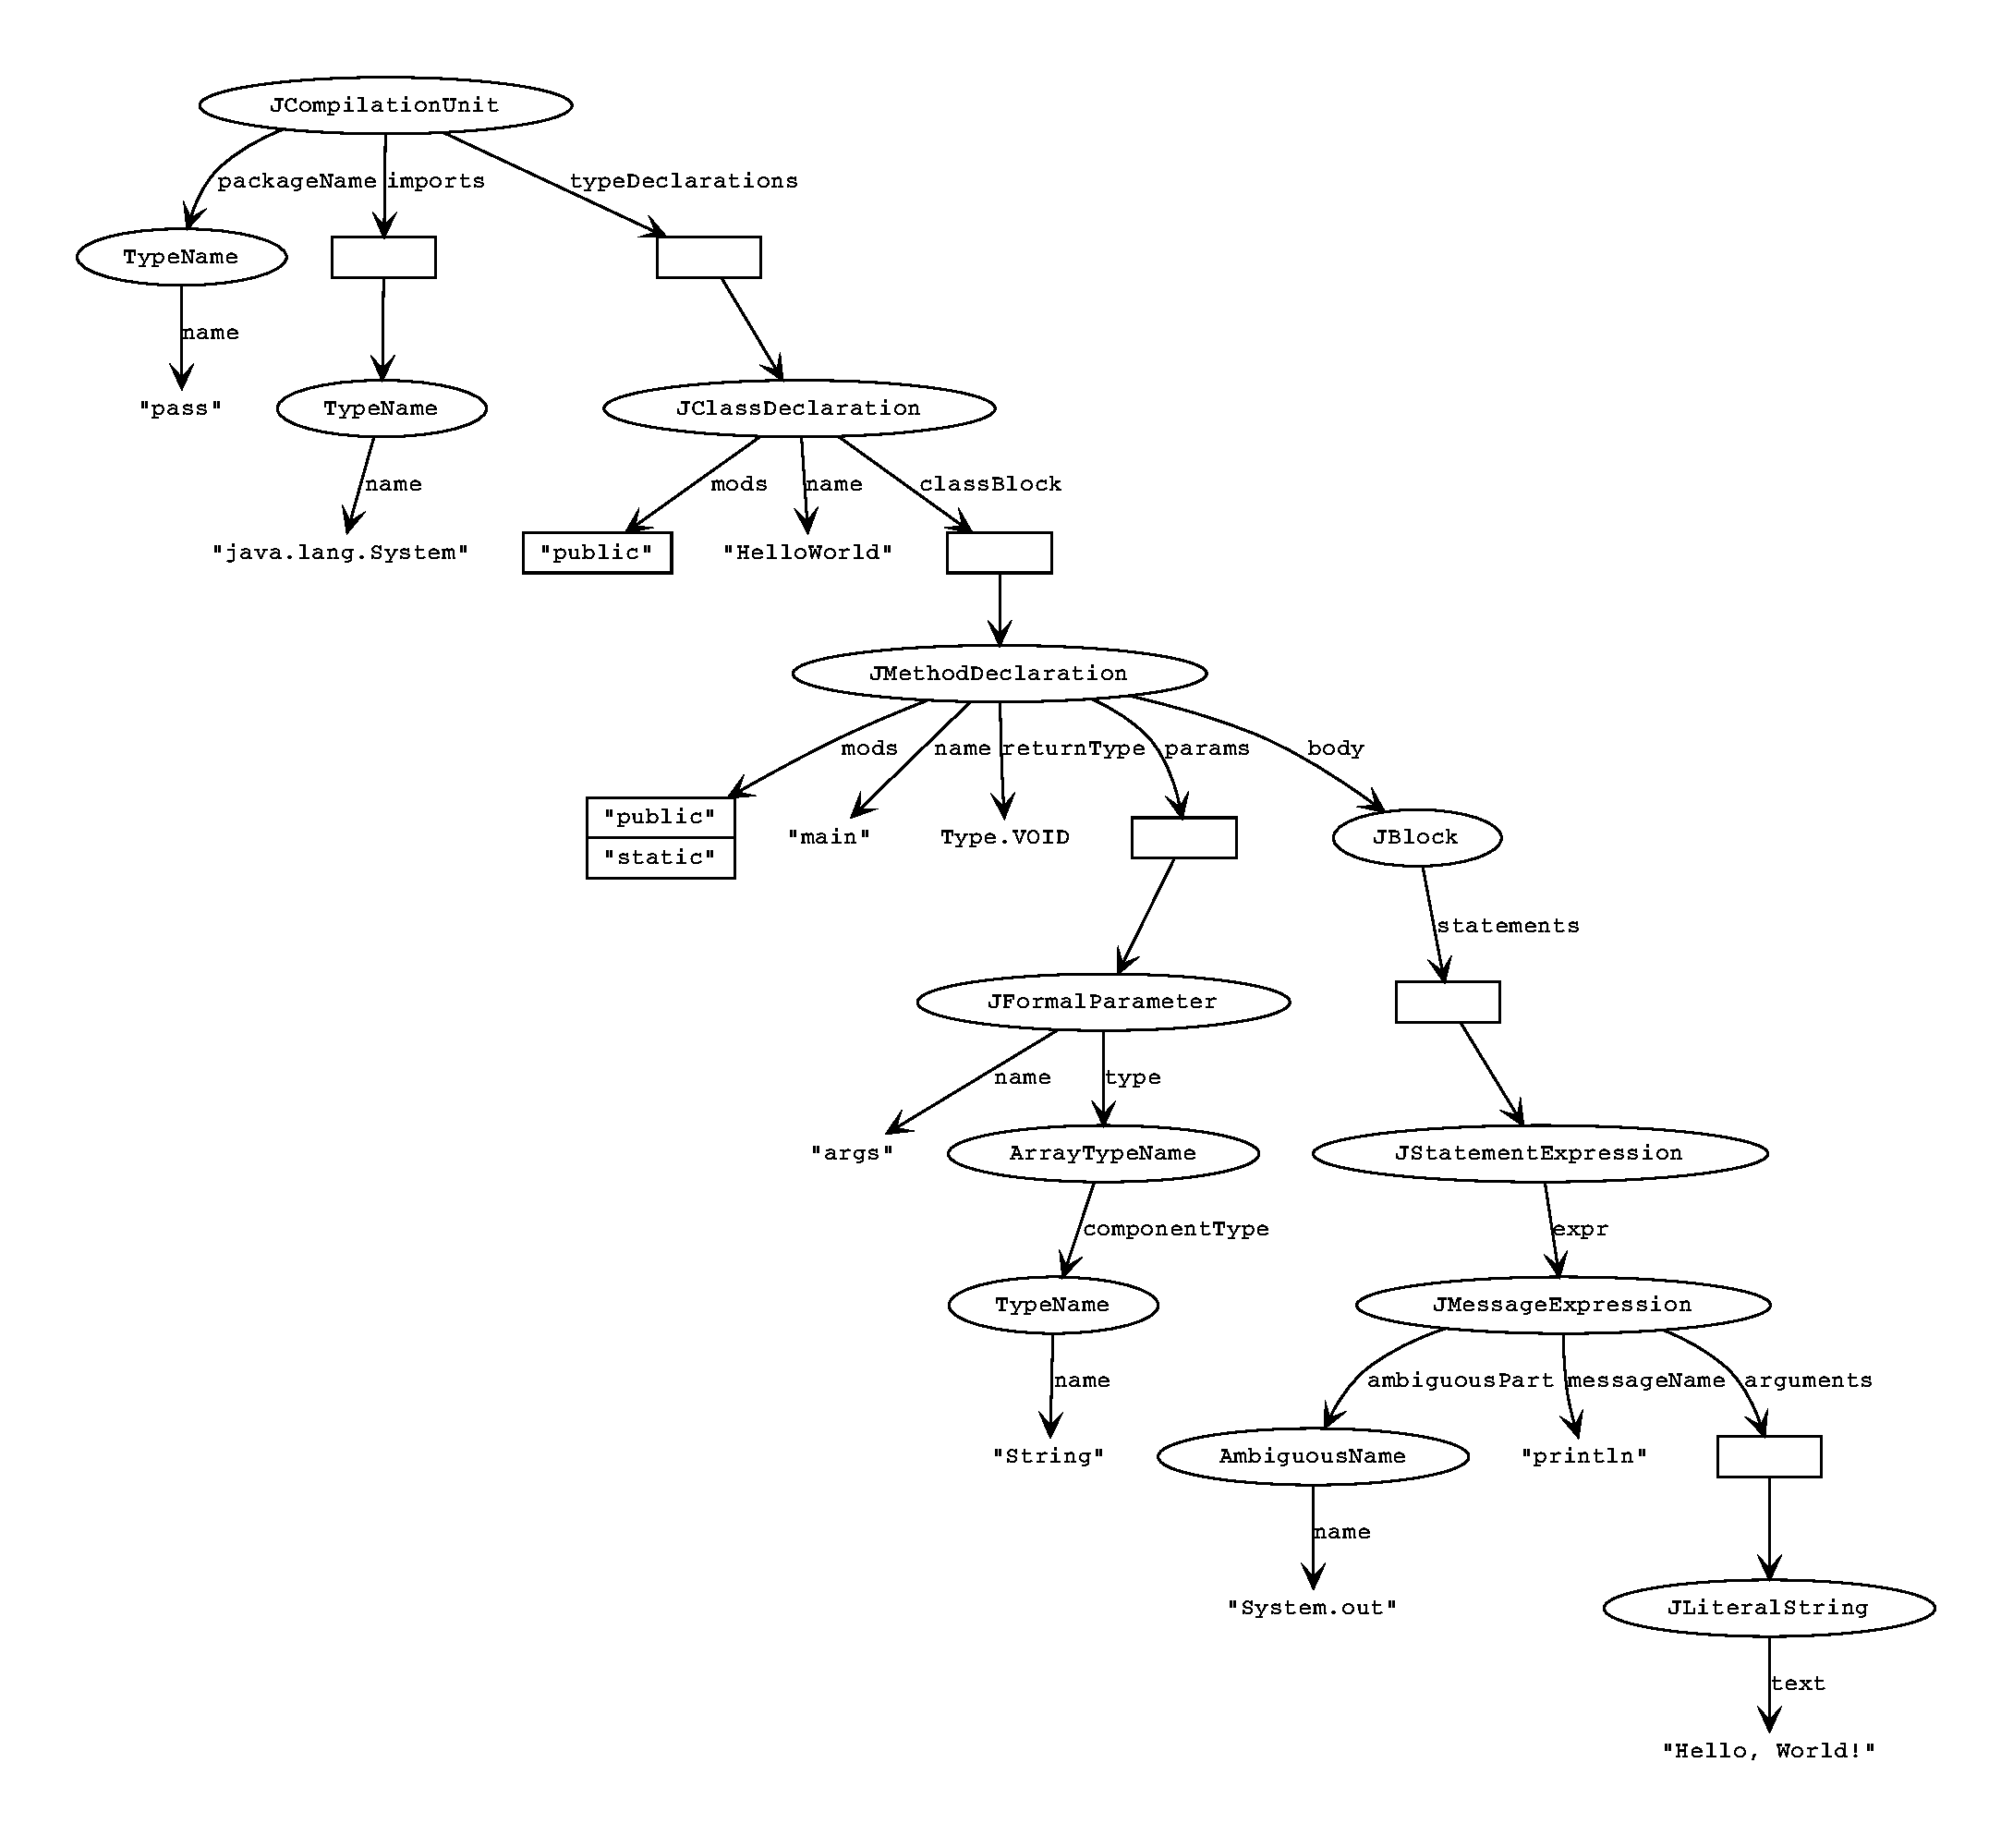
\includegraphics[scale=0.27]{{figures/helloworld_ast}.pdf}}
\end{center}
\end{frame}

\begin{frame}[fragile]
\pause

\jmm (like Java) is statically typed, so it must determine the types of all names and expressions

\pause\bigskip

Types in \jmm are represented using
\begin{itemize}
\pause
\item \lstinline{Type} (wraps \lstinline{java.lang.Class})

\pause
\item \lstinline{Method} (wraps \lstinline{java.lang.reflect.Method})

\pause
\item \lstinline{Constructor} (wraps \lstinline{java.lang.reflect.Constructor})

\pause
\item \lstinline{Field} (wraps \lstinline{java.lang.reflect.Field})

\pause
\item \lstinline{Member} (wraps \lstinline{java.lang.reflect.Member})
\end{itemize}

\pause\bigskip

There are places where \jmm uses \lstinline{TypeName} and \lstinline{ArrayTypeName} to denote a type by its name, before the type is known or defined

\pause\bigskip

An ambiguous expression such as \lstinline{x.y.z} in \lstinline{x.y.z.w()} is denoted as \lstinline{AmbiguousName} by the parser and is reclassified during analysis
\end{frame}

\begin{frame}[fragile]
\pause

\jmm maintains a symbol table (a singly-linked list of \lstinline{Context} objects) in which it declares names

\pause\bigskip

Each object in the symbol table represents some area of scope and contains a mapping from names to definitions

\pause\bigskip

A \lstinline{CompilationUnitContext} object represents the scope comprising the program

\pause\bigskip

A \lstinline{ClassContext} object represents the scope of a class declaration

\pause\bigskip

A \lstinline{LocalContext} object represents the scope of a block

\pause\bigskip

A \lstinline{MethodContext} (subclass of \lstinline{LocalContext}) object represents the scopes of methods and constructors
\end{frame}

\begin{frame}[fragile]
\pause

\lstinline{preAnalyze()} builds the part of the symbol table that is close to the top of the AST, declaring imported types, types introduced by class declarations, and the members in those classes

\pause\bigskip

\lstinline{analyze()} builds the rest of the symbol table, decorating the AST with type information

\pause\bigskip

\lstinline{analyze()} also performs other important tasks such as type checking, accessibility checking, member finding, tree rewriting, and storage allocation
\end{frame}

\begin{frame}[fragile]
\pause

The JVM is a stack machine, meaning all computations are carried out atop the run-time stack

\pause\bigskip

Each time a method is invoked, the JVM
\begin{itemize}
\pause
\item Allocates a stack frame (contiguous block of memory locations) on top of the stack

\pause
\item Assigns positions on the frame for formal parameters and substitutes actual arguments for the parameters

\pause
\item Assigns positions on the frame for values of local variables and temporary results
\end{itemize}

\pause\bigskip

\begin{overprint}
\onslide<7|handout:1>
Stack frame for a static method with $m$ formal parameters and $n$ local variables

\smallskip

\scriptsize{
\begin{center}
\begin{tabular}{R{1.3cm}|C{1.7cm}|} \cline{2-2}
& \makecell{$\vdots$ \\ computations \\ $\vdots$} \\ \cline{2-2}
$m+n-1$ & local variable $n$ \\ \cline{2-2}
& $\vdots$ \\ \cline{2-2}
$m+1$ & local variable $2$ \\ \cline{2-2}
$m$ & local variable $1$ \\ \cline{2-2}
$m-1$ & formal parameter $m$ \\ \cline{2-2}
& $\vdots$ \\ \cline{2-2}
$1$ & formal parameter $2$ \\ \cline{2-2}
$0$ & formal parameter $1$ \\ \cline{2-2}
\end{tabular}
\end{center}
}

\onslide<8|handout:2>
Stack frame for an instance method with $m$ formal parameters and $n$ local variables

\smallskip

\scriptsize{
\begin{center}
\begin{tabular}{R{1.3cm}|C{1.7cm}|} \cline{2-2}
& \makecell{$\vdots$ \\ computations \\ $\vdots$} \\ \cline{2-2}
$m+n$ & local variable $n$ \\ \cline{2-2}
& $\vdots$ \\ \cline{2-2}
$m+2$ & local variable $2$ \\ \cline{2-2}
$m+1$ & local variable $1$ \\ \cline{2-2}
$m$ & formal parameter $m$ \\ \cline{2-2}
& $\vdots$ \\ \cline{2-2}
$2$ & formal parameter $2$ \\ \cline{2-2}
$1$ & formal parameter $1$ \\ \cline{2-2}
$0$ & \texttt{this} \\ \cline{2-2}
\end{tabular}
\end{center}
}
\end{overprint}
\end{frame}

\begin{frame}[fragile]
\pause

The purpose of \lstinline{codegen()} is to generate JVM instructions (aka bytecode)

\pause\bigskip

\lstinline{codegen()} starts at the root of the AST and recursively descends the tree, generating JVM bytecode

\pause\bigskip

\lstinline{CLEmitter} provides an abstraction for the JVM class file

\pause\bigskip

\lstinline{codegen()} in \lstinline{JMethodDeclaration} (AST representation for method declarations)

\begin{overprint}
\onslide<5|handout:1>
\begin{tcolorbox}[enhanced,drop shadow southwest,sharp corners,size=fbox,colback=white,fontlower=\small\ttfamily,collower=silver100]

\begin{lstlisting}[language=Java,style=focusin]
    public void codegen(CLEmitter output) {
        output.addMethod(mods, name, descriptor, null, false);
        if (body != null) {
            body.codegen(output);
        }
        if (returnType == Type.VOID) {
            output.addNoArgInstruction(RETURN);
        }
    }
\end{lstlisting}

\tcblower
\begin{minipage}[t][.25cm][t]{\textwidth}

\end{minipage}
\end{tcolorbox}

\onslide<6|handout:2>
\begin{tcolorbox}[enhanced,drop shadow southwest,sharp corners,size=fbox,colback=white,fontlower=\small\ttfamily,collower=silver900]

\begin{lstlisting}[language=Java,style=focusin,backgroundcolor=\color{lime100}]
    public void codegen(CLEmitter output) {
\end{lstlisting}
\begin{lstlisting}[language=Java,style=focusout]
        output.addMethod(mods, name, descriptor, null, false);
        if (body != null) {
            body.codegen(output);
        }
        if (returnType == Type.VOID) {
            output.addNoArgInstruction(RETURN);
        }
    }
\end{lstlisting}

\tcblower
\begin{minipage}[t][.25cm][t]{\textwidth}
generate code for a method declaration using CLEmitter
\end{minipage}
\end{tcolorbox}

\onslide<7|handout:3>
\begin{tcolorbox}[enhanced,drop shadow southwest,sharp corners,size=fbox,colback=white,fontlower=\small\ttfamily,collower=silver900]

\begin{lstlisting}[language=Java,style=focusout]
    public void codegen(CLEmitter output) {
\end{lstlisting}
\begin{lstlisting}[language=Java,style=focusin,backgroundcolor=\color{lime100}]
        output.addMethod(mods, name, descriptor, null, false);
\end{lstlisting}
\begin{lstlisting}[language=Java,style=focusout]
        if (body != null) {
            body.codegen(output);
        }
        if (returnType == Type.VOID) {
            output.addNoArgInstruction(RETURN);
        }
    }
\end{lstlisting}

\tcblower
\begin{minipage}[t][.25cm][t]{\textwidth}
declare the method
\end{minipage}
\end{tcolorbox}

\onslide<8|handout:4>
\begin{tcolorbox}[enhanced,drop shadow southwest,sharp corners,size=fbox,colback=white,fontlower=\small\ttfamily,collower=silver900]

\begin{lstlisting}[language=Java,style=focusout]
    public void codegen(CLEmitter output) {
        output.addMethod(mods, name, descriptor, null, false);
\end{lstlisting}
\begin{lstlisting}[language=Java,style=focusin,backgroundcolor=\color{lime100}]
        if (body != null) {
            body.codegen(output);
        }
\end{lstlisting}
\begin{lstlisting}[language=Java,style=focusout]
        if (returnType == Type.VOID) {
            output.addNoArgInstruction(RETURN);
        }
    }
\end{lstlisting}

\tcblower
\begin{minipage}[t][.25cm][t]{\textwidth}
generate code for the method body (if any)
\end{minipage}
\end{tcolorbox}

\onslide<9|handout:5>
\begin{tcolorbox}[enhanced,drop shadow southwest,sharp corners,size=fbox,colback=white,fontlower=\small\ttfamily,collower=silver900]

\begin{lstlisting}[language=Java,style=focusout]
    public void codegen(CLEmitter output) {
        output.addMethod(mods, name, descriptor, null, false);
        if (body != null) {
            body.codegen(output);
        }
\end{lstlisting}
\begin{lstlisting}[language=Java,style=focusin,backgroundcolor=\color{lime100}]
        if (returnType == Type.VOID) {
            output.addNoArgInstruction(RETURN);
        }
\end{lstlisting}
\begin{lstlisting}[language=Java,style=focusout]
    }
\end{lstlisting}

\tcblower
\begin{minipage}[t][.25cm][t]{\textwidth}
add implicit RETURN instruction
\end{minipage}
\end{tcolorbox}
\end{overprint}
\end{frame}

\section{The \protect \jmm Compiler Source Tree}
\begin{frame}[fragile]
\pause

The zip file \lstinline{j--.zip} for the base \jmm compiler may be unzipped into any directory (referred to as \lstinline{$j}) of your choosing

\pause\bigskip

The directory \lstinline{$j/j--/src/jminusminus} contains
\begin{itemize}
\pause
\item \lstinline{Main.java}, the driver program

\pause
\item A hand-written scanner (\lstinline{Scanner.java}) and parser (\lstinline{Parser.java})

\pause
\item \lstinline{J*.java} files defining classes representing the AST nodes

\pause
\item \lstinline{CL*.java} files for creating JVM bytecode

\pause
\item \lstinline{S*.java} files for translating JVM bytecode into MIPS code

\pause
\item \lstinline{j--.jj}, the JavaCC specification file for generating (as opposed to hand-writing) a scanner and parser

\pause
\item \lstinline{JavaCCMain}, the driver program that uses the generated scanner and parser

\pause
\item Other Java files providing representation for types and the symbol table
\end{itemize}
\end{frame}

\begin{frame}[fragile]
\pause

Usage syntax for the \jmm compiler (\lstinline{$j/j--/bin/j--})

\begin{tcolorbox}[enhanced,drop shadow southwest,sharp corners,size=fbox,colback=black]
\begin{lstlisting}[style=terminal]
$ sh $j/j--/bin/j--
Usage: j-- <options> <source file>
where possible options include:
  -t Only tokenize input and print tokens to STDOUT
  -p Only parse input and print AST to STDOUT
  -pa Only parse and pre-analyze input and print AST to STDOUT
  -a Only parse, pre-analyze, and analyze input and print AST 
     to STDOUT
  -s <naive|linear|graph> Generate SPIM code
  -r <num> Max. physical registers (1-18) available for 
     allocation; default = 8
  -d <dir> Specify where to place output files; default = .
\end{lstlisting}
\end{tcolorbox}

\pause\bigskip

For example, to just tokenize the \jmm program \lstinline{$j/j--/tests/pass/HelloWorld.java}, run the command

\begin{tcolorbox}[enhanced,drop shadow southwest,sharp corners,size=fbox,colback=black]
\begin{lstlisting}[style=terminal]
$ $j/j--/bin/j-- -t $j/j--/tests/pass/HelloWorld.java
\end{lstlisting}
\end{tcolorbox}

\pause\bigskip

And to compile the program for the JVM, run the command

\begin{tcolorbox}[enhanced,drop shadow southwest,sharp corners,size=fbox,colback=black]
\begin{lstlisting}[style=terminal]
$ $j/j--/bin/j-- $j/j--/tests/pass/HelloWorld.java
\end{lstlisting}
\end{tcolorbox}
\end{frame}

\begin{frame}[fragile]
\pause

\jmm provides an elaborate framework for adding new Java constructs to the \jmm language

\pause\bigskip

For example, to add the division operator (\lstinline{/}) to \jmm, we must
\begin{enumerate}
\pause
\item Modify the \jmm grammar to include the division operator

\pause
\item Modify the scanner to recognize \lstinline{/} as a token

\pause
\item Modify the parser to be able to parse division expressions

\pause
\item Implement type checking (aka semantic analysis) for the division expression

\pause
\item Implement code generation for the division expression
\end{enumerate}

\pause\bigskip

Modify the lexical grammar (\lstinline{$j/j--/lexicalgrammar})

\begin{tcolorbox}[enhanced,drop shadow southwest,sharp corners,size=fbox,colback=white,fontlower=\small\ttfamily,collower=silver900]

\begin{lstlisting}[language={},style=focusin]
// Operators
ASSIGN      ::= "="
...
STAR        ::= "*"
\end{lstlisting}
\begin{lstlisting}[language={},style=focusin,backgroundcolor=\color{lime100}]
DIV         ::= "/"
\end{lstlisting}
\end{tcolorbox}

\pause\bigskip

Modify the syntactic grammar (\lstinline{$j/j--/grammar})

\begin{tcolorbox}[enhanced,drop shadow southwest,sharp corners,size=fbox,colback=white,fontlower=\small\ttfamily,collower=silver900]
\begin{lstlisting}[language={},style=focusin]
multiplicativeExpression ::= unaryExpression // level 2
\end{lstlisting}
\begin{lstlisting}[language={},style=focusin,backgroundcolor=\color{lime100}]
                               {(STAR | DIV) unaryExpression}
\end{lstlisting}
\end{tcolorbox}
\end{frame}

\begin{frame}[fragile]
\pause

Modify the \lstinline{TokenKind} enumeration in \lstinline{TokenInfo.java}

\begin{tcolorbox}[enhanced,drop shadow southwest,sharp corners,size=fbox,colback=white,fontlower=\small\ttfamily,collower=silver900]

\begin{lstlisting}[language=Java,style=focusin]
enum TokenKind {
    EOF ("<EOF>") ,
    ... ,
    STAR ("*") ,
\end{lstlisting}
\begin{lstlisting}[language=Java,style=focusin,backgroundcolor=\color{lime100}]
    DIV ("/") ,
\end{lstlisting}
\begin{lstlisting}[language=Java,style=focusin]
    ...
}
\end{lstlisting}
\end{tcolorbox}

\pause\bigskip

Modify the scanner (\lstinline{Scanner.java})

\begin{tcolorbox}[enhanced,drop shadow southwest,sharp corners,size=fbox,colback=white,fontlower=\small\ttfamily,collower=silver900]

\begin{lstlisting}[language=Java,style=focusin]
if (ch == '/') {
    nextCh();
    if (ch == '/') {
        // CharReader maps all new lines to '\n'
        while (ch != '\n' && ch != EOFCH) {
            nextCh();
        }
    }
    else {
\end{lstlisting}
\begin{lstlisting}[language=Java,style=focusin,backgroundcolor=\color{lime100}]
        return new TokenInfo(DIV, line);
\end{lstlisting}
\begin{lstlisting}[language=Java,style=focusin]
    }
}
\end{lstlisting}
\end{tcolorbox}
\end{frame}


\begin{frame}[fragile]
\onslide<2->
Define a class \lstinline{JDivideOp} in \lstinline{JBinaryExpression.java} to represent an AST node for the division expression

\smallskip

\begin{overprint}
\onslide<2|handout:1>
\begin{tcolorbox}[enhanced,drop shadow southwest,sharp corners,size=fbox,colback=white,fontlower=\small\ttfamily,collower=silver900]

\begin{lstlisting}[language=Java,style=focusin]
class JDivideOp extends JBinaryExpression {
    public JDivideOp(int line, JExpression lhs, JExpression rhs) {
        super(line, "/", lhs, rhs);
    }
 
    public JExpression analyze (Context context) { return this; }
    
    public void codegen(CLEmitter output) { }
}
\end{lstlisting}

\tcblower
\begin{minipage}[t][.25cm][t]{\textwidth}

\end{minipage}
\end{tcolorbox}

\onslide<3|handout:2>
\begin{tcolorbox}[enhanced,drop shadow southwest,sharp corners,size=fbox,colback=white,fontlower=\small\ttfamily,collower=silver900]

\begin{lstlisting}[language=Java,style=focusin]
class JDivideOp extends JBinaryExpression {
\end{lstlisting}
\begin{lstlisting}[language=Java,style=focusin,backgroundcolor=\color{lime100}]
    public JDivideOp(int line, JExpression lhs, JExpression rhs) {
        super(line, "/", lhs, rhs);
    }
\end{lstlisting}
\begin{lstlisting}[language=Java,style=focusin]
 
    public JExpression analyze (Context context) { return this; }
    
    public void codegen(CLEmitter output) { }
}
\end{lstlisting}

\tcblower
\begin{minipage}[t][.25cm][t]{\textwidth}
constructor
\end{minipage}
\end{tcolorbox}

\onslide<4|handout:3>
\begin{tcolorbox}[enhanced,drop shadow southwest,sharp corners,size=fbox,colback=white,fontlower=\small\ttfamily,collower=silver900]

\begin{lstlisting}[language=Java,style=focusin]
class JDivideOp extends JBinaryExpression {
    public JDivideOp(int line, JExpression lhs, JExpression rhs) {
        super(line, "/", lhs, rhs);
    }
 
\end{lstlisting}
\begin{lstlisting}[language=Java,style=focusin,backgroundcolor=\color{lime100}]
    public JExpression analyze (Context context) { return this; }
\end{lstlisting}
\begin{lstlisting}[language=Java,style=focusin]
    
    public void codegen(CLEmitter output) { }
}
\end{lstlisting}

\tcblower
\begin{minipage}[t][.25cm][t]{\textwidth}
for analysis
\end{minipage}
\end{tcolorbox}

\onslide<5|handout:4>
\begin{tcolorbox}[enhanced,drop shadow southwest,sharp corners,size=fbox,colback=white,fontlower=\small\ttfamily,collower=silver900]

\begin{lstlisting}[language=Java,style=focusin]
class JDivideOp extends JBinaryExpression {
    public JDivideOp(int line, JExpression lhs, JExpression rhs) {
        super(line, "/", lhs, rhs);
    }
 
    public JExpression analyze (Context context) { return this; }
    
\end{lstlisting}
\begin{lstlisting}[language=Java,style=focusin,backgroundcolor=\color{lime100}]
    public void codegen(CLEmitter output) { }
\end{lstlisting}
\begin{lstlisting}[language=Java,style=focusin]
}
\end{lstlisting}

\tcblower
\begin{minipage}[t][.25cm][t]{\textwidth}
for code generation
\end{minipage}
\end{tcolorbox}
\end{overprint}
\end{frame}

\begin{frame}[fragile]
\pause\bigskip

Modify the parser (\lstinline{Parser.java})

\begin{tcolorbox}[enhanced,drop shadow southwest,sharp corners,size=fbox,colback=white,fontlower=\small\ttfamily,collower=silver900]
\begin{lstlisting}[language=Java,style=focusin]
private JExpression multiplicativeExpression() {
    int line = scanner.token().line();
    boolean more = true;
    JExpression lhs = unaryExpression();
    while (more) {
        if (have(STAR)) {
            lhs = new JMultiplyOp(line, lhs, unaryExpression());
        }
\end{lstlisting}
\begin{lstlisting}[language=Java,style=focusin,backgroundcolor=\color{lime100}]]
        else if (have(DIV)) {
            lhs = new JDivideOp(line, lhs, unaryExpression());
        }
\end{lstlisting}
\begin{lstlisting}[language=Java,style=focusin]
        else { more = false; }
    }
    return lhs;
}
\end{lstlisting}
\end{tcolorbox}
\end{frame}

\begin{frame}[fragile]
\pause

Implement \lstinline{analyze()} in \lstinline{JDivideOp}

\smallskip

\begin{overprint}
\onslide<2|handout:1>
\begin{tcolorbox}[enhanced,drop shadow southwest,sharp corners,size=fbox,colback=white,fontlower=\small\ttfamily,collower=silver900]

\begin{lstlisting}[language=Java,style=focusin]
public JExpression analyze(Context context) {
    lhs = (JExpression) lhs.analyze(context);
    rhs = (JExpression) rhs.analyze(context);
    lhs.type().mustMatchExpected(line(), Type.INT);
    rhs.type().mustMatchExpected(line(), Type.INT);
    type = Type.INT;
    return this;
}
\end{lstlisting}

\tcblower
\begin{minipage}[t][.25cm][t]{\textwidth}

\end{minipage}
\end{tcolorbox}

\onslide<3|handout:2>
\begin{tcolorbox}[enhanced,drop shadow southwest,sharp corners,size=fbox,colback=white,fontlower=\small\ttfamily,collower=silver900]

\begin{lstlisting}[language=Java,style=focusin,backgroundcolor=\color{lime100}]
public JExpression analyze(Context context) {
\end{lstlisting}
\begin{lstlisting}[language=Java,style=focusout]
    lhs = (JExpression) lhs.analyze(context);
    rhs = (JExpression) rhs.analyze(context);
    lhs.type().mustMatchExpected(line(), Type.INT);
    rhs.type().mustMatchExpected(line(), Type.INT);
    type = Type.INT;
    return this;
}
\end{lstlisting}

\tcblower
\begin{minipage}[t][.25cm][t]{\textwidth}
analyze the expression in the given context
\end{minipage}
\end{tcolorbox}

\onslide<4|handout:3>
\begin{tcolorbox}[enhanced,drop shadow southwest,sharp corners,size=fbox,colback=white,fontlower=\small\ttfamily,collower=silver900]

\begin{lstlisting}[language=Java,style=focusout]
public JExpression analyze(Context context) {
\end{lstlisting}
\begin{lstlisting}[language=Java,style=focusin,backgroundcolor=\color{lime100}]
    lhs = (JExpression) lhs.analyze(context);
    rhs = (JExpression) rhs.analyze(context);
\end{lstlisting}
\begin{lstlisting}[language=Java,style=focusout]
    lhs.type().mustMatchExpected(line(), Type.INT);
    rhs.type().mustMatchExpected(line(), Type.INT);
    type = Type.INT;
    return this;
}
\end{lstlisting}

\tcblower
\begin{minipage}[t][.25cm][t]{\textwidth}
analyze lhs and rhs operands
\end{minipage}
\end{tcolorbox}

\onslide<5|handout:4>
\begin{tcolorbox}[enhanced,drop shadow southwest,sharp corners,size=fbox,colback=white,fontlower=\small\ttfamily,collower=silver900]

\begin{lstlisting}[language=Java,style=focusout]
public JExpression analyze(Context context) {
    lhs = (JExpression) lhs.analyze(context);
    rhs = (JExpression) rhs.analyze(context);
\end{lstlisting}
\begin{lstlisting}[language=Java,style=focusin,backgroundcolor=\color{lime100}]
    lhs.type().mustMatchExpected(line(), Type.INT);
    rhs.type().mustMatchExpected(line(), Type.INT);
\end{lstlisting}
\begin{lstlisting}[language=Java,style=focusout]
    type = Type.INT;
    return this;
}
\end{lstlisting}

\tcblower
\begin{minipage}[t][.25cm][t]{\textwidth}
lhs and rhs must be of type int
\end{minipage}
\end{tcolorbox}

\onslide<6|handout:5>
\begin{tcolorbox}[enhanced,drop shadow southwest,sharp corners,size=fbox,colback=white,fontlower=\small\ttfamily,collower=silver900]

\begin{lstlisting}[language=Java,style=focusout]
public JExpression analyze(Context context) {
    lhs = (JExpression) lhs.analyze(context);
    rhs = (JExpression) rhs.analyze(context);
    lhs.type().mustMatchExpected(line(), Type.INT);
    rhs.type().mustMatchExpected(line(), Type.INT);
\end{lstlisting}
\begin{lstlisting}[language=Java,style=focusin,backgroundcolor=\color{lime100}]
    type = Type.INT;
\end{lstlisting}
\begin{lstlisting}[language=Java,style=focusout]
    return this;
}
\end{lstlisting}

\tcblower
\begin{minipage}[t][.25cm][t]{\textwidth}
type of the expression is int
\end{minipage}
\end{tcolorbox}

\onslide<7|handout:6>
\begin{tcolorbox}[enhanced,drop shadow southwest,sharp corners,size=fbox,colback=white,fontlower=\small\ttfamily,collower=silver900]
\begin{lstlisting}[language=Java,style=focusout]
public JExpression analyze(Context context) {
    lhs = (JExpression) lhs.analyze(context);
    rhs = (JExpression) rhs.analyze(context);
    lhs.type().mustMatchExpected(line(), Type.INT);
    rhs.type().mustMatchExpected(line(), Type.INT);
    type = Type.INT;
\end{lstlisting}
\begin{lstlisting}[language=Java,style=focusin,backgroundcolor=\color{lime100}]
    return this;
\end{lstlisting}
\begin{lstlisting}[language=Java,style=focusout]
}
\end{lstlisting}

\tcblower
\begin{minipage}[t][.25cm][t]{\textwidth}
return the analyzed expression
\end{minipage}
\end{tcolorbox}

\end{overprint}
\end{frame}

\begin{frame}[fragile]
\pause

Implement \lstinline{codegen()} in \lstinline{JDivideOp}

\smallskip

\begin{overprint}
\onslide<2|handout:1>

\begin{tcolorbox}[enhanced,drop shadow southwest,sharp corners,size=fbox,colback=white,fontlower=\small\ttfamily,collower=silver900]

\begin{lstlisting}[language=Java,style=focusin]
public void codegen(CLEmitter output) {
    lhs.codegen(output);
    rhs.codegen(output);
    output.addNoArgInstruction(IDIV);
}
\end{lstlisting}

\tcblower
\begin{minipage}[t][.25cm][t]{\textwidth}

\end{minipage}
\end{tcolorbox}

\onslide<3|handout:2>
\begin{tcolorbox}[enhanced,drop shadow southwest,sharp corners,size=fbox,colback=white,fontlower=\small\ttfamily,collower=silver900]

\begin{lstlisting}[language=Java,style=focusin,backgroundcolor=\color{lime100}]
public void codegen(CLEmitter output) {
\end{lstlisting}
\begin{lstlisting}[language=Java,style=focusout]
    lhs.codegen(output);
    rhs.codegen(output);
    output.addNoArgInstruction(IDIV);
}
\end{lstlisting}

\tcblower
\begin{minipage}[t][.25cm][t]{\textwidth}
generate code for the expression using CLEmitter
\end{minipage}
\end{tcolorbox}

\onslide<4|handout:3>
\begin{tcolorbox}[enhanced,drop shadow southwest,sharp corners,size=fbox,colback=white,fontlower=\small\ttfamily,collower=silver900]

\begin{lstlisting}[language=Java,style=focusout]
public void codegen(CLEmitter output) {
\end{lstlisting}
\begin{lstlisting}[language=Java,style=focusin,backgroundcolor=\color{lime100}]
    lhs.codegen(output);
    rhs.codegen(output);
\end{lstlisting}
\begin{lstlisting}[language=Java,style=focusout]
    output.addNoArgInstruction(IDIV);
}
\end{lstlisting}

\tcblower
\begin{minipage}[t][.25cm][t]{\textwidth}
generate code for lhs and rhs operands
\end{minipage}
\end{tcolorbox}

\onslide<5|handout:4>
\begin{tcolorbox}[enhanced,drop shadow southwest,sharp corners,size=fbox,colback=white,fontlower=\small\ttfamily,collower=silver900]

\begin{lstlisting}[language=Java,style=focusout]
public void codegen(CLEmitter output) {
    lhs.codegen(output);
    rhs.codegen(output);
\end{lstlisting}
\begin{lstlisting}[language=Java,style=focusin,backgroundcolor=\color{lime100}]
    output.addNoArgInstruction(IDIV);
\end{lstlisting}
\begin{lstlisting}[language=Java,style=focusout]
}
\end{lstlisting}

\tcblower
\begin{minipage}[t][.25cm][t]{\textwidth}
generate code for the division operation
\end{minipage}
\end{tcolorbox}

\end{overprint}
\end{frame}

\begin{frame}[fragile]
\pause

Write a test \jmm program \lstinline{Division.java} (say under \lstinline{$j/j--/tests})

\begin{tcolorbox}[enhanced,drop shadow southwest,sharp corners,size=fbox,colback=white,fontlower=\small\ttfamily,collower=silver900]

\begin{lstlisting}[language=Java,style=focusin]
import java.lang.Integer;
import java.lang.System;

public class Division {
    public static void main(String[] args) {
        int a = Integer.parseInt(args[0]);
        int b = Integer.parseInt(args[1]);
        System.out.println(a / b);
    }
}
\end{lstlisting}
\end{tcolorbox}

\pause\bigskip

To compile the changes to the \jmm compiler, go to \lstinline{$j/j--}, and run

\begin{tcolorbox}[enhanced,drop shadow southwest,sharp corners,size=fbox,colback=black]
\begin{lstlisting}[style=terminal]
$ ant clean compile jar
\end{lstlisting}
\end{tcolorbox}

\pause\bigskip

To compile the test program using the \jmm, run

\begin{tcolorbox}[enhanced,drop shadow southwest,sharp corners,size=fbox,colback=black]
\begin{lstlisting}[style=terminal]
$ sh ./bin/j-- tests/Division.java
\end{lstlisting}
\end{tcolorbox}

\pause\bigskip

To run the test program (\lstinline{Division.class}), run

\begin{tcolorbox}[enhanced,drop shadow southwest,sharp corners,size=fbox,colback=black]
\begin{lstlisting}[style=terminal]
$ java Division 42 6
7
\end{lstlisting}
\end{tcolorbox}
\end{frame}
\end{document}
